\chapter{\ifenglish Background Knowledge and Theory\else ทฤษฎีที่เกี่ยวข้อง\fi}


การทำโครงงาน เริ่มต้นด้วยการศึกษาค้นคว้า ทฤษฎีที่เกี่ยวข้อง หรือ งานวิจัย/โครงงาน ที่เคยมีผู้นำเสนอไว้แล้ว ซึ่งเนื้อหาในบทนี้ก็จะเกี่ยวกับการอธิบายถึงสิ่งที่เกี่ยวข้องกับโครงงาน เพื่อให้ผู้อ่านเข้าใจเนื้อหาในบทถัดๆ ไปได้ง่ายขึ้น


\section{ทฤษฎีที่เป็นความรู้ในการขนส่งแบบติดตามอุณหภูมิ }

\begin{enumerate}
    \item ระบบทำความเย็น (Cooling System): การลดและรักษาระดับอุณหภูมิหรือการทำความเย็น เพื่อ	ให้สภาพแวดล้อมหรือพื้นที่จัดเก็บมีความเหมาะสมในการเก็บรักษาและขนส่งสินค้า โดยให้ความ		สำคัญกับอุณหภูมิ, ความชื้น และความเข้าใจในสินค้า เพื่อเลือกใช้วิธีการทำความเย็นที่เหมาะสม 	เช่น การใช้น้ำแข็ง, น้ำเย็น, การแช่แข็ง หรือการใช้ระบบสูญญากาศ 
    \item คลังสินค้าห้องเย็น (Cold Storage): พื้นที่จัดเก็บสินค้าที่มีการควบคุมอุณหภูมิภายในให้เหมาะสม 	สำหรับการจัดเก็บสินค้าในช่วงระยะเวลาหนึ่งก่อนการกระจายหรือขนส่งสินค้า เพื่อรักษาคุณภาพ	สินค้าในสภาพแวดล้อมที่มีอุณหภูมิและความชื้นคงที่ โดยทั่วไปอุุณหภูมิภายในคลังสินค้าห้องเย็นจะ	ต่ำกว่า 25 องศาเซลเซียส หรืออาจติดลบ ขึ้นอยู่กับประเภทของสินค้าที่จัดเก็บ
    \item การขนส่งแบบควบคุมอุณหภูมิ (Cold Transpot): การใช้ยานพาหนะที่ออกแบบมาเฉพาะสำหรับ	การขนส่งที่ต้องการติดตาม หรือควบคุมอุณหภูมิ เช่น รถบรรทุกห้องเย็น ที่มีระบบควบคุมอุณหภูมิ	และความชื้นภายใน เพื่อรักษาคุณภาพ และความสดใหม่ของสินค้าระหว่างการขนส่ง
    \item การจัดการโลจิสติกส์โซ่ความเย็น (Cold Chain Management): การวางแผน และควบคุม		กระบวนการทั้งหมดในห่วงโซ่อุปทาน ตั้งแต่การผลิต, การจัดเก็บ, การขนส่ง จนถึงการจัดจำหน่าย 	เพื่อให้สินค้าที่ต้องการควบคุมอุณหภูมิได้รับการดูแลอย่างเหมาะสม
    \item การติดตามและควบคุมอุณหภูมิระหว่างการขนส่ง: การใช้เทคโนโลยี เช่น IoTs และเซนเซอร์วัด		อุณหภูมิ เพื่อตรวจสอบ และบันทึกอุณหภูมิในบรรจุภัณฑ์ที่จัดเก็บสินค้าตลอดระยะเวลาในการขนส่ง	เพื่อให้มมั่นใจว่าสินค้าได้รับการควบคุมอุณหภูมิตามที่กำหนด
    \item การเลือกบรรณจุภัณฑ์ที่เหมาะสมสำหรับการขนส่งควบคุมอุณหภูมิ: การเลือกบรรจุภัณฑ์ที่ีเหมาะสม	เป็นสิ่งสำคัญในการรักษาคุณภาพของสินค้าในระหว่างการขนส่งควบคุมอุณหภูมิ โดยควรมีคุณสมบัติ	ดังนี้
        \begin{itemize}
            \item ความแข็งแรงและทนทาน : เพื่อป้องกันความเสียหายจากแรงกระแทกหรือการกดทับระหว่างการขนส่ง
            \item การป้องกันการรั่วซึม : เพื่อป้องกันการปนเปื้อนจากน้ำ สารเคมี หรือสิ่งสกปรก
            \item ขนาดที่เหมาะสม : เพื่อให้สินค้าเหมาะกับบรรจุภัณฑ์ ไม่แน่นหรือหลวมเกินไป
            \item วัสดุที่ได้รับมาตรฐาน Food Grade : เพื่อความปลอดภัยของผู้บริโภค
        \end{itemize}
    \item การใช้บรรจุภัณฑ์โซ่ความเย็น (Cold Chain Packaging): บรรจุภัณฑ์โซ่ความเย็นถูกออกแบบมาเพื่อ	รักษาอุณหภูมิของสินค้าที่ไวต่อความร้อนในระหว่างการขนส่ง การเลือกใช้บรรจุภัณฑ์เหล่านี้ช่วยลด	ความเสี่ยงในการเสื่อมสภาพของสินค้าและรักษาคุณภาพของผลิตภัณฑ์ 
\end{enumerate}

\section{Blockchain – Hyperledger Fabric }
Hyperledger Fabric เป็นเฟรมเวิร์กบล็อกเชนแบบโอเพ่นซอร์สที่พัฒนาโดยโครงการ Hyperledger ภายใต้การดูแลของ Linux Foundation ออกแบบมาเพื่อการใช้งานในระดับองค์กร  
โดยมีสถาปัตยกรรมแบบโมดูลาร์ที่ช่วยให้สามารถปรับแต่งและขยายระบบได้ตามความต้องการของธุรกิจ 
โดยมีคุณสมบัติเด่นดังนี้ 

\begin{enumerate}
    \item สถาปัตยกรรมแบบโมดูลาร์: ช่วยให้สามารถปรับแต่งส่วนประกอบต่าง ๆ เช่น ฉันทามติ (consensus) และบริการสมาชิก (membership services) เพื่อให้เหมาะสมกับการใช้งานเฉพาะด้าน
    \item การรองรับธุรกรรมที่เป็นความลับ: ด้วยการใช้ช่องทาง (channels) ทำให้สามารถแบ่งปันข้อมูลเฉพาะกับผู้เข้าร่วมที่เกี่ยวข้องเท่านั้น ซึ่งเหมาะสำหรับธุรกิจที่ต้องการความเป็นส่วนตัวสูง 
\end{enumerate}
จากคุณสมบัติต่าง ๆ ข้างต้น เราจึงได้นำ Hyperledger Fabric มาประยุกต์ใช้กับโครงงานดังนี้ 
\begin{enumerate}
    \item การติดตามสินค้า: บล็อกเชนสามารถบันทึกข้อมูลการขนส่งสินค้า เช่น ปริมาณสินค้า สถานที่ และเวลา ทำให้ทุกฝ่ายที่เกี่ยวข้องสามารถตรวจสอบสถานะสินค้าได้แบบเรียลไทม์ 
    \item การตรวจสอบอุณหภูมิ: สำหรับสินค้าที่ต้องการควบคุมอุณหภูมิ เช่น ยา อาหารทะเล หรือผลิตภัณฑ์จากนม การบันทึกข้อมูลอุณหภูมิในบล็อกเชนช่วยให้มั่นใจว่าสินค้าได้รับการจัดเก็บและขนส่งในสภาพแวดล้อมที่เหมาะสม 
    \item ความโปร่งใสและความน่าเชื่อถือ: การใช้บล็อกเชนช่วยให้ข้อมูลการขนส่งไม่สามารถถูกแก้ไขได้ ทำให้ผู้บริโภคและผู้เกี่ยวข้องมั่นใจในคุณภาพและความปลอดภัยของสินค้า
\end{enumerate}

จากการเลือกใช้ Hyperledger Fabric จึงทำให้เกิดประโยชน์ต่าง ๆ มากมายในโครงงานนี้เช่น การลดความซับซ้อนของกระบวนการด้วยการรวบรวมข้อมูลทั้งหมดไว้ในระบบเดียว ทำให้สามารถลดขั้นตอนการประสานงานระหว่างฝ่ายต่าง ๆ และด้วยคุณสมบัติของ Blockchain ที่ข้อมูลไม่สามารถแก้ไขได้ ทำให้สามารถลดความเสี่ยงจากการทุจริตหรือข้อผิดพลาดได้อีกด้วย 
\begin{itemize}
    \item ข้อดี: Hyperledger Fabric เป็น Permissioned Blockchain ที่รองรับ Private Channels ทำให้สามารถกำหนดสิทธิ์การเข้าถึงข้อมูลเฉพาะกลุ่มที่เกี่ยวข้องได้ ช่วยเพิ่มความปลอดภัยและความเป็นส่วนตัวของข้อมูล
    \item ข้อเสีย: โครงสร้างที่ซับซ้อนและต้องมีการตั้งค่าหลายส่วน เช่น Peer Nodes, Orderers และ Membership Services ทำให้การติดตั้งและดูแลระบบต้องใช้ความเชี่ยวชาญเฉพาะด้าน
\end{itemize}

\section{KidBright Board}
\begin{figure}[H]
    \begin{center}
        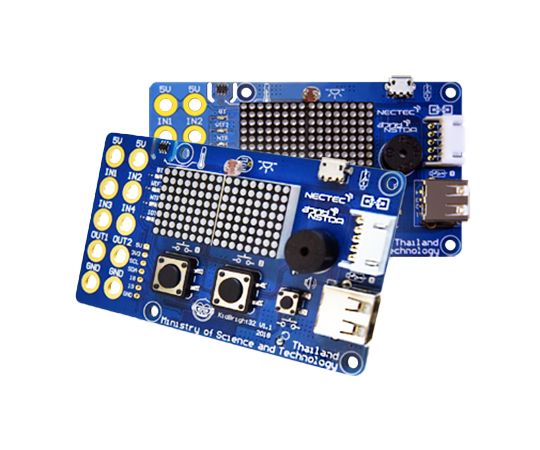
\includegraphics[width=1\textwidth]{chapters/kidbright-transparent.png}
    \end{center}
    \caption[KidBright Board]{KidBright Board}
\end{figure}
KidBright เป็นบอร์ดไมโครคอนโทรลเลอร์ที่พัฒนาโดยคนไทย มีวัตถุประสงค์เพื่อส่งเสริมการเรียนรู้ด้านการเขียนโปรแกรมและอิเล็กทรอนิกส์ในกลุ่มนักเรียนและผู้สนใจ บอร์ดนี้มาพร้อมกับเซ็นเซอร์และอุปกรณ์พื้นฐาน เช่น เซ็นเซอร์วัดแสง (LDR), เซ็นเซอร์วัดอุณหภูมิ, ปุ่มกด, และจอแสดงผล LED 16x8 ทำให้ผู้ใช้สามารถเริ่มต้นพัฒนาโครงการได้ทันที
\begin{itemize}
    \item ข้อดี: KidBright Board เป็นไมโครคอนโทรลเลอร์ที่ออกแบบมาให้ใช้งานง่าย มีฟังก์ชันพื้นฐานในตัว เช่น จอ LED, ปุ่มกด และพอร์ตเชื่อมต่ออุปกรณ์เสริม รองรับการเขียนโปรแกรมแบบบล็อก (Block-based Programming) และภาษา Python ทำให้สามารถพัฒนาโครงงานได้อย่างรวดเร็ว
    \item ข้อเสีย: KidBright Board มีข้อจำกัดด้านประสิทธิภาพเมื่อเทียบกับไมโครคอนโทรลเลอร์ระดับสูง เช่น Raspberry Pi หรือ ESP32 โดยเฉพาะในด้านการประมวลผลข้อมูลจำนวนมากหรือการเชื่อมต่ออินเทอร์เน็ตแบบไร้สาย
\end{itemize}

\section{เซนเซอร์ DS18B20 }
\begin{figure}[H]
    \begin{center}
        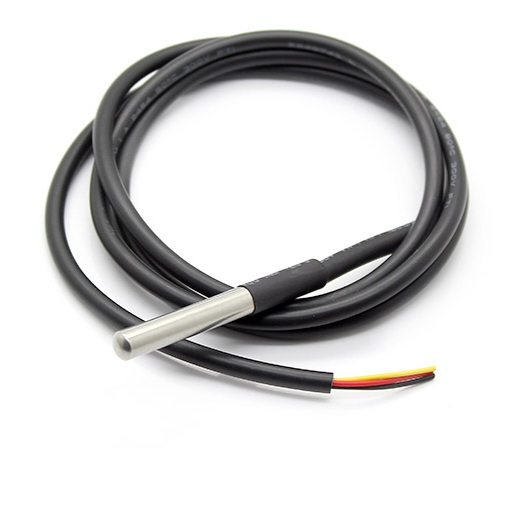
\includegraphics[width=1\textwidth]{chapters/k6xejr.jpg}
    \end{center}
    \caption[เซนเซอร์ DS18B20 ]{เซนเซอร์ DS18B20 }
\end{figure}
DS18B20 เป็นเซ็นเซอร์วัดอุณหภูมิแบบดิจิตอลที่ได้รับความนิยม เนื่องจากความแม่นยำและความสะดวกในการใช้งาน เซ็นเซอร์นี้สามารถวัดอุณหภูมิในช่วง -55°C ถึง +125°C และมีความละเอียดที่ปรับได้ตั้งแต่ 9 ถึง 12 บิต นอกจากนี้ DS18B20 ยังรองรับการเชื่อมต่อแบบ 1-Wire ซึ่งช่วยลดจำนวนสายที่ต้องใช้ในการเชื่อมต่อ
\begin{itemize}
    \item ข้อดี: DS18B20 เป็นเซ็นเซอร์วัดอุณหภูมิแบบดิจิทัลที่มีความแม่นยำสูง รองรับช่วงอุณหภูมิกว้างตั้งแต่ -55°C ถึง +125°C และสามารถสื่อสารผ่านโปรโตคอล 1-Wire ซึ่งช่วยลดจำนวนสายสัญญาณที่ใช้ในการเชื่อมต่อ
    \item ข้อเสีย: เซ็นเซอร์ DS18B20 มีอัตราการตอบสนองที่ช้ากว่าเซ็นเซอร์ประเภทอื่น เช่น เทอร์มิสเตอร์ หรือ RTD ทำให้ไม่เหมาะกับการวัดอุณหภูมิที่ต้องการการเปลี่ยนแปลงแบบเรียลไทม์
\end{itemize}

\section{\ifenglish%
\ifcpe CPE \else ISNE \fi knowledge used, applied, or integrated in this project
\else%
ความรู้ตามหลักสูตรซึ่งถูกนำมาใช้หรือบูรณาการในโครงงาน
\fi
}

ในการพัฒนาโครงงานนี้ได้นำองค์ความรู้จากรายวิชาต่าง ๆ มาประยุกต์ใช้ให้สามารถออกแบบและพัฒนาระบบได้อย่างมีประสิทธิภาพ โดยรายวิชาที่เกี่ยวข้องมีดังนี้
\begin{itemize}
    \item 261207 ฺBasic Computer Engineering Laboratory: นำความรู้เกี่ยวกับการพัฒนาเว็บไซต์โดยใช้ทั้ง JavaScript และ TypeScript รวมถึงการดึงข้อมูลจาก API และหลักการของ HTTP method มาประยุกต์ใช้ในการพัฒนา Front-End และ Back-End ของโครงงานนี้
    \item 261343 Database System Laboratory: นำความรู้เกี่ยวกับการจัดการฐานข้อมูล รวมถึงการใช้งาน Docker ซึ่งเป็นส่วนสำคัญในการสร้างและจัดการ Blockchain ซึ่งเป็นฐานข้อมูลหลักของโครงงานนี้
    \item 261215 Embedded System Laboratory: นำความรู้ในรายวิชานี้มาใช้เพื่อออกแบบชิ้นงานของโครงงาน รวมไปถึงการประดิษฐ์ชิ้นงาน และการเลือกใช้งานบอร์ดหรือเซนเซอร์
    \item 261430 Wireless Network: นำความรู้เกี่ยวกับ Kidbright board ที่ได้เรียนในใช้เรียนเป็นเหตุผลหลักในการเลือกใช้บอร์ดนี้ในโครงงาน
    \item 261200 Object-Oriented Programming: นำแนวคิดเชิงวัตถุมาใช้ในการออกแบบและพัฒนาโครงสร้างต่าง ๆ ในระบบ
    \item 261361 Software Engineering: นำความรู้ในวิชานี้มาวิเคราะห์ความต้องการของผู้ใช้งาน, วางแผนโครงสร้างของระบบ, วางแผนการพัฒนาโครงสร้างของระบบ และ การทดสอบระบบต่าง ๆ ในโครงงานนี้
\end{itemize}
\section{\ifenglish%
Extracurricular knowledge used, applied, or integrated in this project
\else%
ความรู้นอกหลักสูตรซึ่งถูกนำมาใช้หรือบูรณาการในโครงงาน
\fi
}

โครงงานนี้ได้นำความรู้จากแหล่งอื่น ๆ ที่ไม่ได้อยู่ในรายวิชาเรียนหรือหลักสูตรของภาควิชา เพื่อเพิ่มประสิทธิภาพและเสริมสร้างความสามารถของการทำโครงงาน โดยมีรายละเอียดดังนี้
\begin{itemize}
    \item Blockchain – Hyperledger Fabric: โครงงานนี้ได้นำความรู้เกี่ยวกับ Hyperledger Fabric ซึ่งเป็นหนึ่งในเฟรมเวิร์กของ Permissioned Blockchain มาใช้ในการพัฒนาและออกแบบระบบที่เกี่ยวข้องกับการติดตามข้อมูลและการจัดเก็บบันทึกที่มีความปลอดภัยสูง โดยความรู้ที่นำมาใช้ประกอบด้วย
    \begin{enumerate}
        \item โครงสร้างของ Hyperledger Fabric: ระบบที่รองรับการทำงานแบบโมดูลาร์ สามารถกำหนดกลไกการยืนยันตัวตน (Identity Management) และรูปแบบฉันทามติ (Consensus Mechanism) ได้ตามต้องการ
        \item การใช้ Smart Contract (Chaincode): Chaincode ใน Hyperledger Fabric ทำหน้าที่เหมือน Smart Contract ในบล็อกเชนอื่น ๆ โดยใช้ภาษา Go, Node.js หรือ Java ซึ่งช่วยให้สามารถกำหนดตรรกะของธุรกรรมที่เกิดขึ้นในระบบได้
        \item Private Channels และ Data Privacy: Hyperledger Fabric รองรับการสร้าง Private Channels ซึ่งช่วยให้เฉพาะบางองค์กรในเครือข่ายสามารถเข้าถึงข้อมูลที่เกี่ยวข้องได้ เพิ่มความปลอดภัยและความเป็นส่วนตัวของข้อมูล
        \item การจัดเก็บข้อมูลแบบ Distributed Ledger: ทำให้ข้อมูลมีความถูกต้อง เชื่อถือได้ และไม่สามารถแก้ไขย้อนหลังได้ง่าย ซึ่งช่วยเพิ่มความโปร่งใสของข้อมูลที่บันทึกในระบบ
        \item การเชื่อมต่อ Hyperledger Fabric กับอุปกรณ์ IoT: ใช้สำหรับรับข้อมูลจากเซ็นเซอร์ DS18B20 และส่งเข้าสู่ระบบบล็อกเชนเพื่อบันทึกข้อมูลอุณหภูมิในลักษณะที่ปลอดภัยและตรวจสอบได้
    \end{enumerate}
    การนำ Hyperledger Fabric มาใช้ในโครงงานนี้ช่วยเพิ่มความน่าเชื่อถือของข้อมูล ลดโอกาสการปลอมแปลง และทำให้สามารถตรวจสอบข้อมูลย้อนหลังได้อย่างแม่นยำ
\end{itemize}
\begin{itemize}
    \item โครงงานนี้ได้นำความรู้ด้านระบบคลาวด์คอมพิวติ้ง (Cloud Computing) ของ Amazon Web Services มาประยุกต์ใช้เป็นโครงสร้างพื้นฐาน (Infrastructure) หลักของระบบ เพื่อรองรับการติดตั้งและประมวลผลเครือข่าย Permissioned Blockchain (Hyperledger Fabric) รวมถึงเซิร์ฟเวอร์ตัวกลาง (Middleware) สำหรับการพัฒนาและออกแบบระบบติดตามข้อมูลและจัดเก็บบันทึกที่มีความปลอดภัยสูงและทำงานได้อย่างมีเสถียรภาพ โดยความรู้ที่นำมาประยุกต์ใช้ประกอบด้วย
    \begin{enumerate}
        \item โครงสร้างพื้นฐาน AWS Global Infrastructure :
โครงสร้างพื้นฐานระดับโลกของ AWS ประกอบด้วยส่วนสำคัญดังนี้
•	AWS Regions คือพื้นที่ทางภูมิศาสตร์ที่ AWS ตั้งศูนย์ข้อมูล ปัจจุบันมีมากกว่า 30 Regions ทั่วโลก แต่ละ Region ประกอบด้วย Availability Zones หลายแห่งที่แยกจากกันทางกายภาพ
•	Availability Zones (AZs) คือศูนย์ข้อมูลที่แยกเป็นอิสระต่อกันภายใน Region เดียวกัน ออกแบบมาเพื่อความทนทานต่อความล้มเหลว (Fault Tolerance) โดยมีการเชื่อมต่อกันด้วยเครือข่ายความเร็วสูงและ Latency ต่ำ
•	Edge Locations คือโหนดที่กระจายอยู่ทั่วโลกสำหรับบริการ Amazon CloudFront เพื่อให้บริการเนื้อหาในตำแหน่งที่ใกล้กับผู้ใช้งานที่สุด

        \item บริการหลักของ AWS ที่เกี่ยวข้องกับโครงการ
โครงการนี้ได้นำบริการหลัก ๆ ของ AWS มาใช้งาน ได้แก่
Amazon EC2 (Elastic Compute Cloud)
Amazon EC2 เป็นบริการ IaaS ที่ให้ความสามารถในการสร้างเซิร์ฟเวอร์เสมือน (Virtual Machines) หรือที่เรียกว่า Instance บน Cloud ผู้ใช้งานสามารถเลือกขนาดของ Instance ตามความต้องการและปรับขนาดได้ตามการใช้งาน EC2 รองรับระบบปฏิบัติการหลายประเภท เช่น Linux, Windows และ macOS
Instance Types ของ EC2 แบ่งออกเป็นหลายกลุ่มตามวัตถุประสงค์การใช้งาน เช่น General Purpose (t3, m5), Compute Optimized (c5), Memory Optimized (r5), Storage Optimized (i3) และ Accelerated Computing (p3, g4)
Amazon S3 (Simple Storage Service)
Amazon S3 เป็นบริการจัดเก็บข้อมูลแบบ Object Storage ที่มีความทนทาน (Durability) สูงถึง 99.999999999% โดยข้อมูลจะถูกเก็บในรูปแบบ Object ภายใน Bucket ซึ่งสามารถเก็บข้อมูลได้ไม่จำกัดจำนวน
S3 มี Storage Classes หลายประเภทสำหรับตอบสนองความต้องการการเข้าถึงข้อมูลที่แตกต่างกัน ได้แก่ S3 Standard สำหรับข้อมูลที่เข้าถึงบ่อย, S3 Intelligent-Tiering สำหรับข้อมูลที่รูปแบบการเข้าถึงไม่แน่นอน, S3 Glacier สำหรับการเก็บข้อมูลระยะยาวและการ Archive
Amazon RDS (Relational Database Service)
Amazon RDS เป็นบริการฐานข้อมูลเชิงสัมพันธ์แบบ Managed Service ที่ช่วยลดภาระการดูแลจัดการฐานข้อมูล รองรับ Database Engine หลายประเภท เช่น MySQL, PostgreSQL, MariaDB, Oracle, Microsoft SQL Server และ Amazon Aurora
คุณสมบัติสำคัญของ RDS ได้แก่ การ Backup อัตโนมัติ, การ Patch อัตโนมัติ, Multi-AZ Deployment สำหรับ High Availability, Read Replicas สำหรับเพิ่มประสิทธิภาพการอ่านข้อมูล และการเข้ารหัสข้อมูลทั้งแบบ At-rest และ In-transit
AWS Lambda
AWS Lambda เป็นบริการ Serverless Computing ที่ช่วยให้นักพัฒนาสามารถรันโค้ดโดยไม่ต้องจัดการเซิร์ฟเวอร์ Lambda จะทำงานเมื่อมี Event เกิดขึ้น และจะหยุดทำงานเมื่อโค้ดทำงานเสร็จสิ้น ผู้ใช้งานจ่ายค่าบริการเฉพาะเวลาที่โค้ดทำงานจริงเท่านั้น
Lambda รองรับภาษาโปรแกรมหลายภาษา เช่น Python, Node.js, Java, Go, C\#, Ruby และ PowerShell มักถูกนำมาใช้ร่วมกับ Amazon API Gateway เพื่อสร้าง RESTful API หรือใช้ในรูปแบบ Event-driven Architecture
Amazon VPC (Virtual Private Cloud)
Amazon VPC ช่วยให้ผู้ใช้งานสามารถสร้างเครือข่ายเสมือนที่แยกจากกันบน AWS Cloud โดยมีการควบคุม IP Address Range, Subnets, Route Tables และ Network Gateways VPC เป็นพื้นฐานสำคัญของการออกแบบ Network Architecture ที่ปลอดภัยบน AWS
ส่วนประกอบสำคัญของ VPC ได้แก่ Public Subnet และ Private Subnet, Internet Gateway สำหรับการเชื่อมต่ออินเทอร์เน็ต, NAT Gateway สำหรับให้ Private Subnet เข้าถึงอินเทอร์เน็ต, Security Groups และ Network Access Control Lists (NACLs) สำหรับควบคุมการเข้าถึง
AWS IAM (Identity and Access Management)
AWS IAM เป็นบริการจัดการสิทธิ์การเข้าถึงทรัพยากรบน AWS ช่วยให้สามารถกำหนดว่าใครสามารถเข้าถึงทรัพยากรใดได้บ้าง IAM ใช้แนวคิด Principle of Least Privilege ซึ่งหมายความว่าผู้ใช้งานหรือบริการจะได้รับสิทธิ์เฉพาะที่จำเป็นสำหรับการทำงานเท่านั้น
IAM ประกอบด้วย Users, Groups, Roles และ Policies โดย Policies เขียนในรูปแบบ JSON เพื่อกำหนด Actions, Resources และ Conditions ที่อนุญาตหรือปฏิเสธการเข้าถึง

        \item AWS DevOps และการ Deploy แอปพลิเคชัน DevOps เป็นแนวปฏิบัติที่รวม Development และ Operations เข้าด้วยกัน โดยมีเป้าหมายเพื่อเพิ่มความเร็วในการพัฒนา ปรับปรุงคุณภาพซอฟต์แวร์ และเพิ่มความน่าเชื่อถือของการ Deploy AWS มีบริการที่รองรับกระบวนการ DevOps อย่างครบครัน
AWS CodePipeline
AWS CodePipeline เป็นบริการ Continuous Integration และ Continuous Delivery (CI/CD) ที่ช่วยอัตโนมัติขั้นตอนการ Build, Test และ Deploy แอปพลิเคชัน ช่วยให้สามารถส่งมอบ Feature ใหม่และอัปเดตอย่างรวดเร็วและเชื่อถือได้
Amazon ECS และ Amazon EKS
Amazon Elastic Container Service (ECS) เป็นบริการ Container Orchestration ที่รองรับ Docker Container ช่วยให้สามารถรันและจัดการ Container บน AWS ได้ง่าย ในขณะที่ Amazon Elastic Kubernetes Service (EKS) เป็นบริการ Managed Kubernetes ที่ช่วยลดความซับซ้อนในการจัดการ Kubernetes Cluster
AWS CloudFormation
AWS CloudFormation เป็นบริการ Infrastructure as Code (IaC) ที่ช่วยให้สามารถกำหนดและ Provision โครงสร้างพื้นฐาน AWS โดยใช้ Template ในรูปแบบ JSON หรือ YAML ทำให้สามารถจัดการโครงสร้างพื้นฐานได้อย่างสม่ำเสมอและทำซ้ำได้

        \item ความปลอดภัยบน AWS:
AWS ให้ความสำคัญกับความปลอดภัยเป็นลำดับแรก โดยใช้โมเดล Shared Responsibility Model ซึ่งแบ่งความรับผิดชอบด้านความปลอดภัยระหว่าง AWS และลูกค้า AWS รับผิดชอบความปลอดภัยของโครงสร้างพื้นฐาน Cloud (Security of the Cloud) ในขณะที่ลูกค้ารับผิดชอบความปลอดภัยของสิ่งที่ทำงานอยู่บน Cloud (Security in the Cloud)
AWS Shield และ AWS WAF
AWS Shield เป็นบริการป้องกัน DDoS Attack โดยอัตโนมัติ แบ่งเป็น Shield Standard ที่ให้บริการฟรีสำหรับทุก AWS Customer และ Shield Advanced สำหรับการป้องกันขั้นสูง AWS Web Application Firewall (WAF) ช่วยป้องกัน Web Application จาก Exploit และ Bot ที่พยายามโจมตีช่องโหว่
AWS KMS (Key Management Service)
AWS KMS เป็นบริการจัดการ Encryption Key สำหรับการเข้ารหัสข้อมูล รวมเข้ากับบริการอื่น ๆ ของ AWS ได้อย่างราบรื่น ช่วยให้สามารถควบคุมการเข้าถึง Key และตรวจสอบการใช้งาน Key ผ่าน AWS CloudTrail


        \item การ Monitoring และ Logging บน AWS
การ Monitoring และ Logging เป็นส่วนสำคัญของการดูแลระบบบน Cloud AWS มีบริการที่ครอบคลุมสำหรับการตรวจสอบและวิเคราะห์ประสิทธิภาพของระบบ
Amazon CloudWatch
Amazon CloudWatch เป็นบริการ Monitoring และ Observability สำหรับ AWS ให้ข้อมูล Metrics, Logs และ Events ของทรัพยากร AWS สามารถตั้งค่า Alarm เพื่อแจ้งเตือนเมื่อ Metric เกินค่าที่กำหนด และสร้าง Dashboard เพื่อแสดงภาพรวมของระบบได้
AWS CloudTrail
AWS CloudTrail บันทึก API Call ทั้งหมดที่เกิดขึ้นใน AWS Account ช่วยให้สามารถตรวจสอบการกระทำต่าง ๆ ที่เกิดขึ้นกับทรัพยากร AWS ได้ เป็นเครื่องมือสำคัญสำหรับ Security Auditing, Compliance และ Troubleshooting

    \end{enumerate}
    จากการศึกษาทฤษฎีและเทคโนโลยีที่เกี่ยวข้อง พบว่า Amazon Web Services (AWS) เป็นแพลตฟอร์ม Cloud Computing ที่มีความสมบูรณ์และครอบคลุมบริการที่หลากหลาย ตั้งแต่การประมวลผล การจัดเก็บข้อมูล ฐานข้อมูล ระบบเครือข่าย ไปจนถึงความปลอดภัยและการ Monitoring
โครงสร้างพื้นฐานระดับโลกของ AWS ที่ประกอบด้วย Regions และ Availability Zones ช่วยให้ระบบมีความพร้อมใช้งานสูง (High Availability) และรองรับการขยายตัวได้อย่างยืดหยุ่น บริการต่าง ๆ ของ AWS ที่นำมาใช้ในโครงการนี้ ได้แก่ EC2, S3, RDS, Lambda, VPC และ IAM ล้วนเป็นบริการที่ได้รับการยอมรับอย่างกว้างขวางในอุตสาหกรรมและมีเอกสารอ้างอิงที่ครอบคลุม ซึ่งเป็นพื้นฐานสำคัญในการพัฒนาโครงการนี้ให้มีประสิทธิภาพและเชื่อถือได้

\end{itemize}